\question You are celebrating Christmas with your family when suddenly the power goes out and all of the Christmas lights go off. Not to fear, because you learned in your physics class how to generate power! Using an assembly of refrigerator magnets, you create a uniform magnetic field with a magnitude of 2 T. You then assemble a very long circuit with a movable bar of length $L=10$ cm sliding along the frictionless circuit, like the one shown in the figure. The magnetic field is perpendicular to this circuit and points out of the page. Your plan is to tie a string to the bar and pull it to produce a current through a single Christmas tree bulb, which requires 0.5 W of power to illuminate and has a resistance of 10 $\Omega$. How fast do you need to pull the bar in order to light the bulb?

\begin{figure}[ht!]
	\centering
	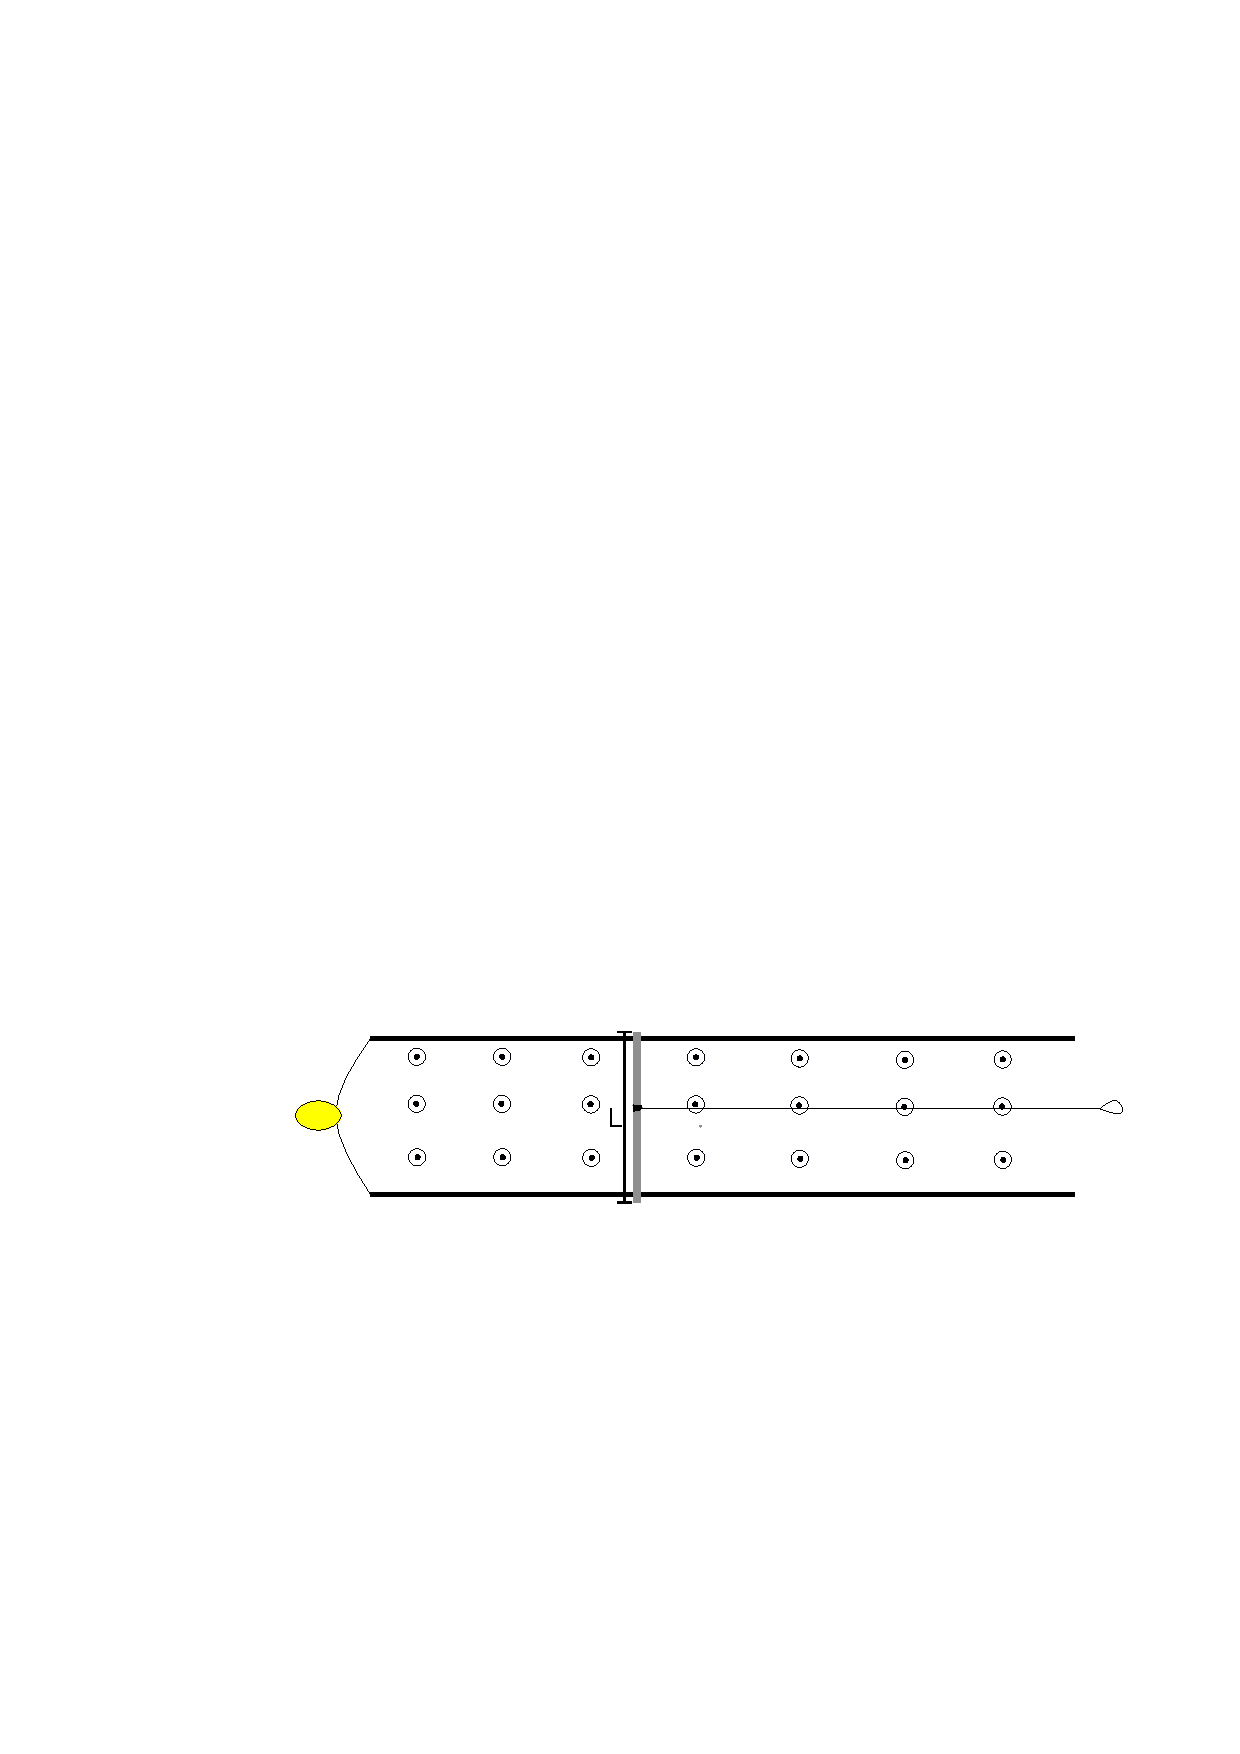
\includegraphics[width=12cm]{motional_emf.pdf}
\end{figure} 